\section{Ablation Studies}
\label{sec:ablation_studies}

Ablation studies evaluated three components of the RECIST-guided lesion segmentation pipeline: backbone architecture, auxiliary anatomy supervision, and adaptive field-of-view expansion with AutoZoom. These controlled ablations used shorter training runs and smaller crops than the final model, so they should be interpreted as component comparisons rather than direct final-model results. Additional setup details are provided in Appendix~\ref{app:controlled_ablation_details}.


\subsection{Architecture Ablation}
\label{sec:architecture_ablation}

Five segmentation backbones were compared using the controlled protocol described in Appendix~\ref{app:controlled_ablation_details}. Auxiliary anatomy supervision was disabled for this comparison.

Table~\ref{tab:architecture_ablation_main} shows the 49-case validation results. MedNeXt-v2 f32 achieved the best validation score, with \(71.40\), compared with \(65.08\) for the next-best backbone, SwinUNETR f24. In the paired comparison, this corresponded to an improvement of \(+6.32\) percentage points, with a 95\% bootstrap CI of \([+3.90,+8.80]\) percentage points. MedNeXt-v2 f32 was therefore selected as the final segmentation backbone.

\begin{table}[htbp]
\centering
\caption{
Matched architecture ablation on the 49-case validation set.
}
\label{tab:architecture_ablation_main}
\begin{tabular}{lcccc}
\toprule
\textbf{Backbone} & \textbf{Params.} & \textbf{Score (\%)} & \textbf{DSC (\%)} & \textbf{NSD (\%)} \\
\midrule
UNet base         & 1.19M  & 63.90 & 70.87 & 56.92 \\
SegResNet         & 4.70M  & 63.59 & 72.13 & 55.06 \\
SwinUNETR f24     & 15.70M & 65.08 & 72.32 & 57.84 \\
MedNeXt-v2 small  & 1.28M  & 65.04 & 72.16 & 57.92 \\
\textbf{MedNeXt-v2 f32}
                  & \textbf{6.92M}
                  & \textbf{71.40}
                  & \textbf{76.06}
                  & \textbf{66.74} \\
\bottomrule
\end{tabular}
\end{table}

\subsection{Auxiliary Anatomy Supervision}
\label{sec:auxiliary_head_ablation}

The auxiliary head was evaluated using a matched 15-epoch control experiment described in Appendix~\ref{app:auxiliary_head_control}. 
The comparison tested whether enabling the PanTS auxiliary anatomy--tumor head improved RECIST-guided lesion segmentation.

Table~\ref{tab:aux_head_ablation_main} reports the best-threshold validation results. 
Auxiliary supervision improved the mean validation score by \(+0.96\) percentage points, but the 95\% bootstrap confidence interval included zero \([-0.18,+2.05]\). 
The auxiliary head is therefore interpreted as a weak training-time regularizer rather than a definitive improvement or standalone anatomy segmentation component.

\begin{table}[htbp]
\centering
\caption{
Auxiliary-head ablation using a matched MedNeXt-v2 small prompt setup.
Metrics are reported as mean \(\pm\) SD over the 49-case validation set on a \(0\)--\(100\) scale.
}
\label{tab:aux_head_ablation_main}
\begin{tabular}{lcccc}
\toprule
\textbf{Variant} & \textbf{Threshold} & \textbf{Score (\%)} & \textbf{DSC (\%)} & \textbf{NSD (\%)} \\
\midrule
No auxiliary head
& 0.35
& \(66.13 \pm 13.09\)
& \(72.63 \pm 11.18\)
& \(59.63 \pm 18.45\) \\
PanTS auxiliary head
& 0.35
& \(\mathbf{67.09 \pm 13.29}\)
& \(\mathbf{73.39 \pm 11.08}\)
& \(\mathbf{60.80 \pm 18.68}\) \\
\midrule
Paired improvement
& --
& \(+0.96 \pm 4.01\)
& \(+0.76 \pm 3.15\)
& \(+1.17 \pm 5.21\) \\
\bottomrule
\end{tabular}
\end{table}

Additional threshold-sweep results are provided in Appendix~\ref{app:auxiliary_head_control}.

\subsection{AutoZoom}
\label{sec:autozoom_ablation}

Table~\ref{tab:autozoom_ablation} compares fixed RECIST-centered regional crop inference with adaptive AutoZoom. 
The table reports the mean challenge score on a \(0\)--\(100\) scale, where \(\Delta\) denotes AutoZoom minus fixed-crop inference in percentage points. 
AutoZoom triggered in only a small fraction of cases and had near-neutral aggregate performance. 
On the validation set, the difference was small, with a 95\% bootstrap CI spanning zero \([-0.32,+0.02]\) percentage points. 
AutoZoom is therefore best interpreted as a selective fallback for cases where the initial RECIST-centered crop may truncate the target lesion.

\begin{table}[htbp]
\centering
\caption{
AutoZoom ablation. 
Scores denote the mean challenge score on a \(0\)--\(100\) scale. 
\(\Delta\) is reported as AutoZoom minus fixed-crop inference in percentage points.
``Largest'' refers to the largest PanTS targets by lesion size.
}
\label{tab:autozoom_ablation}
\setlength{\tabcolsep}{5pt}
\renewcommand{\arraystretch}{1.05}
{\small
\begin{tabular}{lrrrrr}
\toprule
\multirow{2}{*}{\textbf{Subset}} 
& \multirow{2}{*}{\textbf{\(N\)}} 
& \multirow{2}{*}{\textbf{Triggers}} 
& \multicolumn{2}{c}{\textbf{Challenge score (\%)}} 
& \multirow{2}{*}{\textbf{\(\Delta\) (pp)}} \\
\cmidrule(lr){4-5}
& & & \textbf{Fixed crop} & \textbf{AutoZoom} & \\
\midrule
Largest 10     & 10  & 1 \; (10.0\%) & 62.46 & 63.51 & +1.05 \\
Largest 40     & 40  & 5 \; (12.5\%) & 57.03 & 58.05 & +1.02 \\
Largest 120    & 120 & 7 \; (5.8\%)  & 63.91 & 64.34 & +0.43 \\
All PanTS      & 801 & 23 \; (2.9\%) & 64.10 & 64.19 & +0.09 \\
Validation set & 49  & 3 \; (6.1\%)  & 75.99 & 75.87 & -0.12 \\
\bottomrule
\end{tabular}
}
\end{table}

Adaptive expansion was retained to improve robustness in context-limited cases rather than to increase average validation performance. 
The largest-lesion subsets showed small positive changes, while the full validation set showed a slight decrease. 
These results suggest that AutoZoom can recover missed lesion extent when additional field of view is needed, but may also reduce segmentation quality when the expanded crop lowers the effective spatial resolution.

Figure~\ref{fig:autozoom_examples} shows qualitative validation examples. 
Adaptive expansion recovered missed lesion extent in some cases, but reduced segmentation quality in others.

\begin{figure}[htbp]
    \centering
    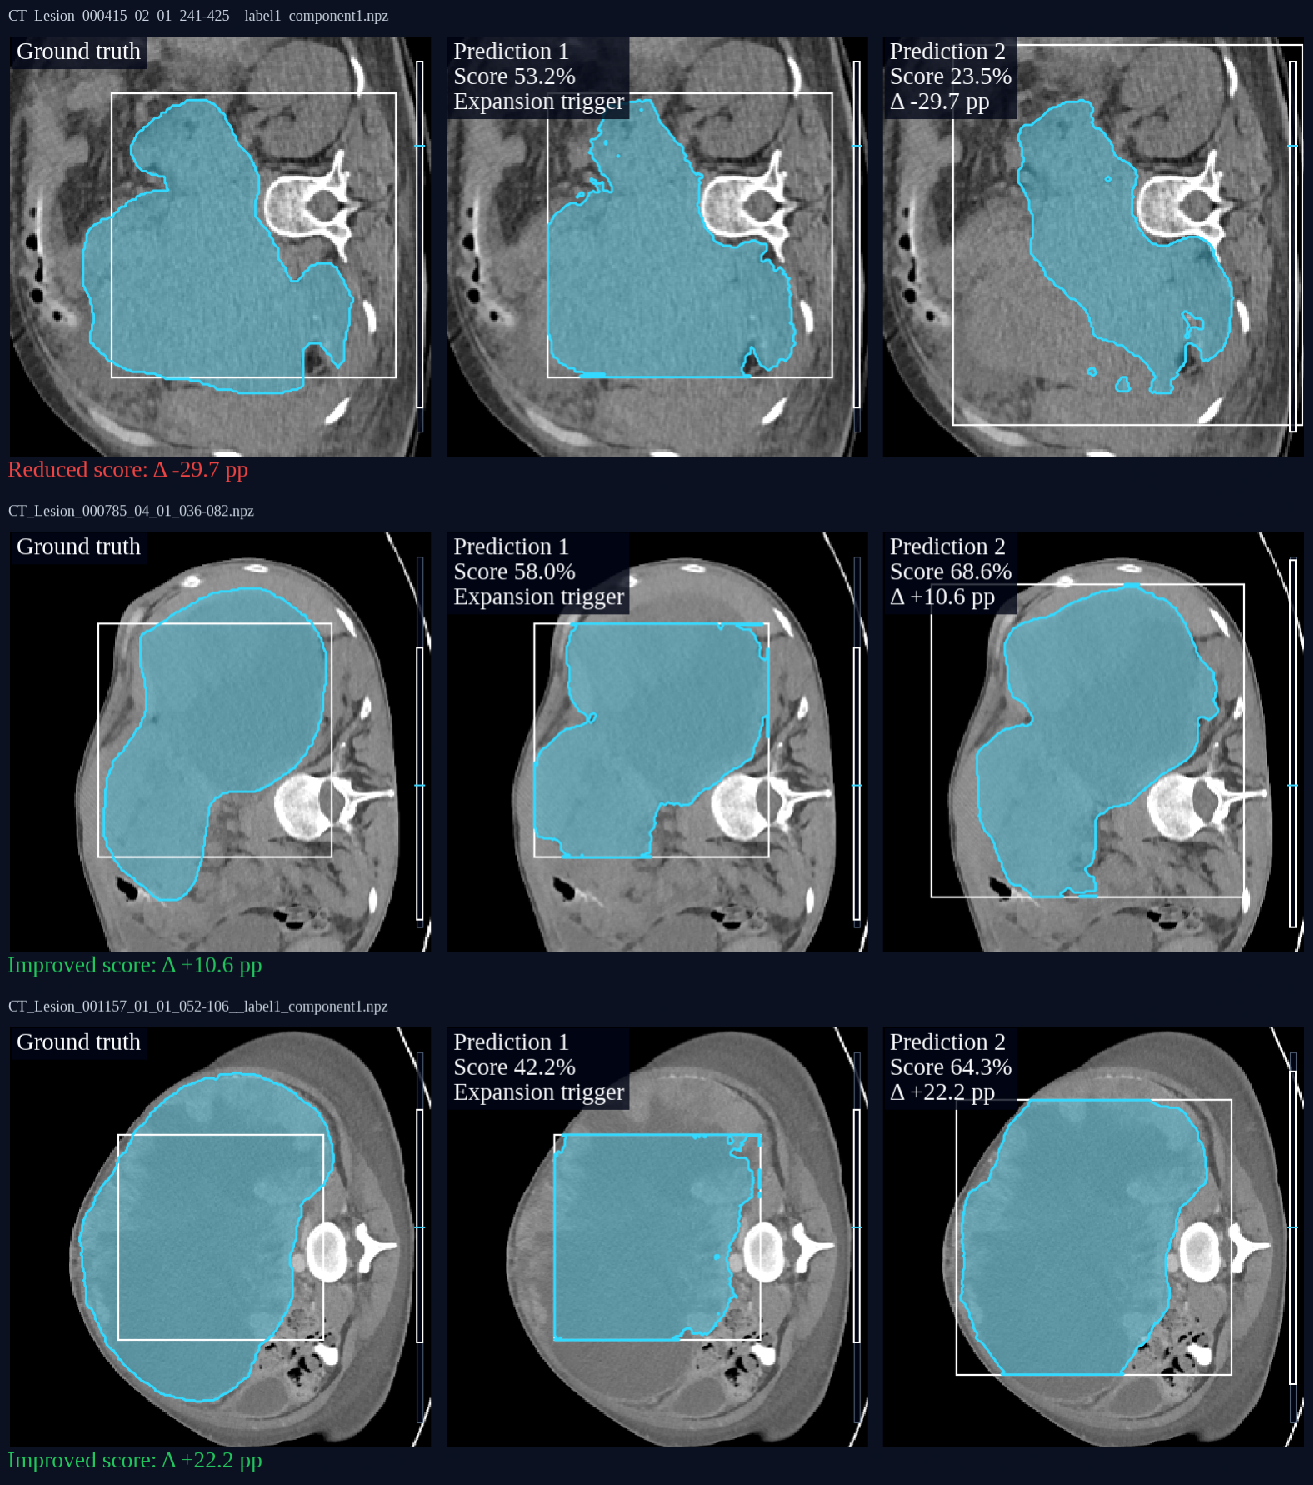
\includegraphics[width=\linewidth]{images/task2_autozoom_xy_validation_selected_v2.pdf}
    \caption{
    Qualitative examples of RECIST-guided AutoZoom on the validation set.
    Each row shows the ground truth, the first prediction using the initial crop, and the second prediction after adaptive crop expansion.
    }
    \label{fig:autozoom_examples}
\end{figure}